%Danilo
%===========================================
%  6.explica su interpretación dentro del modelo.
%===========================================


\begin{frame}{Interpretación Geométrica}

    \begin{columns}[c]

        %========================================
        % COLUMNA IZQUIERDA
        %========================================
        \column{0.50\textwidth}

        \begin{block}{Relación entre distancia y amplitud}

            \small

            Mientras menor sea la distancia entre la fuente y un sensor, mayor será la amplitud registrada por dicho sensor.

            \vspace{0.2cm}

            Por eso, la distancia $R_i$ se convierte en una variable fundamental dentro del modelo matemático.

        \end{block}

        \vspace{0.25cm}

        \begin{block}{Idea física}

            \small

            La señal se atenúa al propagarse, de modo que los sensores más alejados registran amplitudes menores.

        \end{block}

        \vspace{0.15cm}

        \begin{center}
            \small
            \textbf{
            La geometría espacial controla el comportamiento de las amplitudes sísmicas.
            }
        \end{center}

        %========================================
        % COLUMNA DERECHA
        %========================================
        \column{0.46\textwidth}

        \begin{center}
            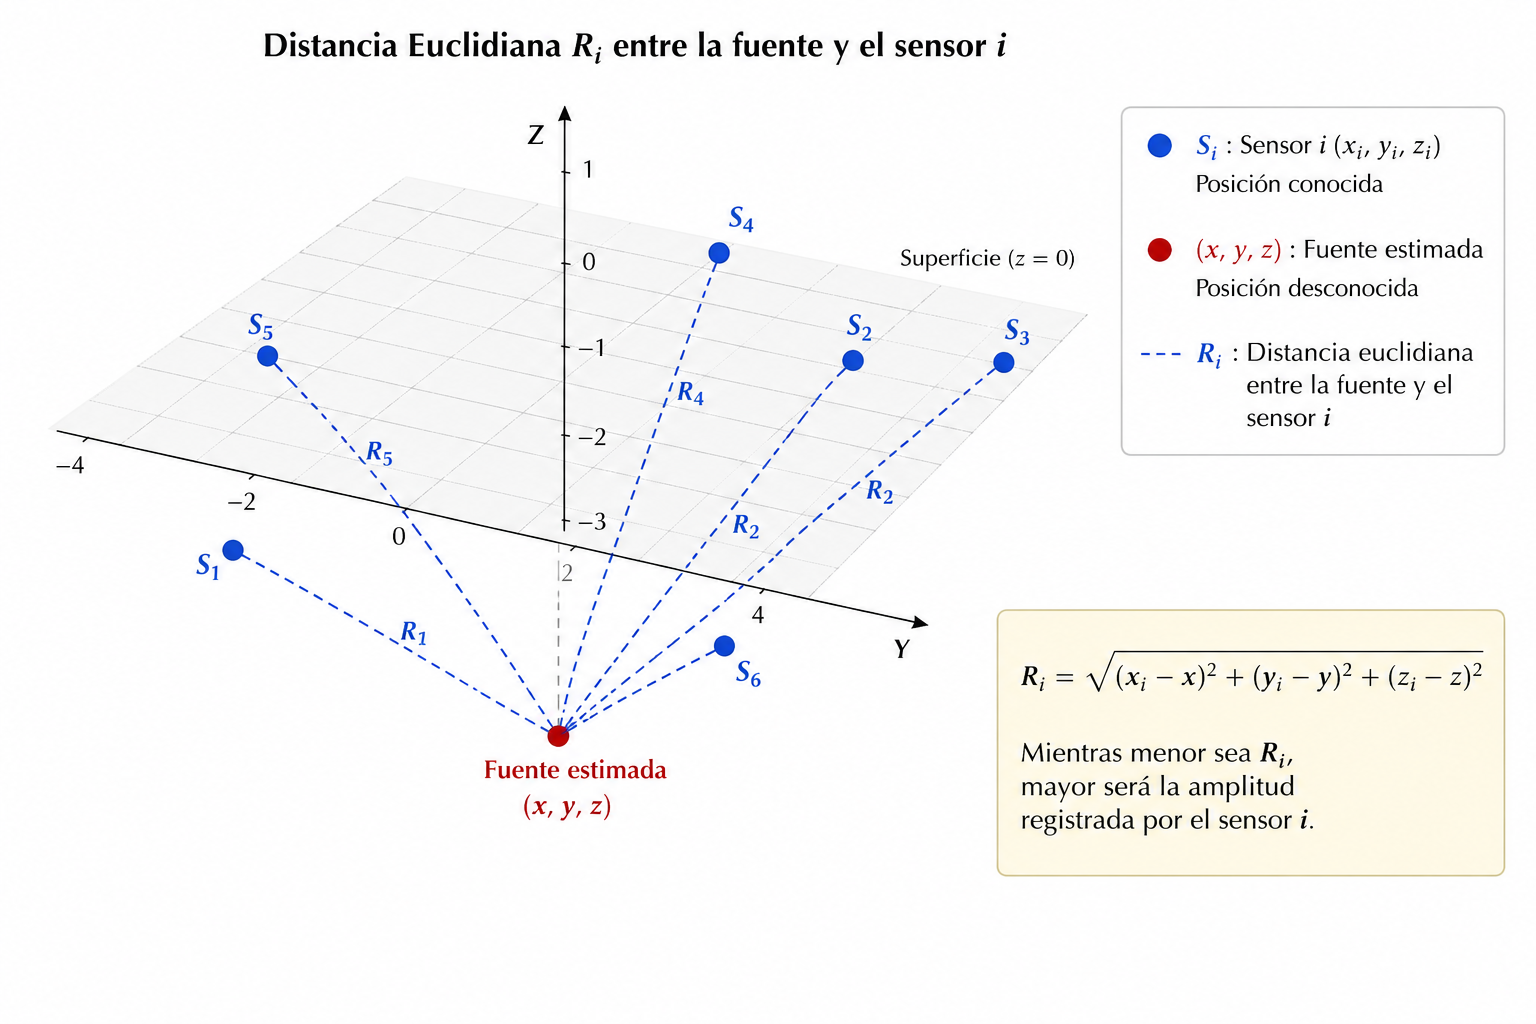
\includegraphics[width=\textwidth]{Imagenes/DistanciaEuclidiana3D.png}
        \end{center}

        \vspace{0.15cm}

        \begin{center}
            \tiny
            \textcolor{gray}{
            La posición de la fuente modifica las distancias $R_i$ y, en consecuencia, las amplitudes predichas por el modelo.
            }
        \end{center}

    \end{columns}

\end{frame}